\documentclass[]{article}

% Imported Packages
%------------------------------------------------------------------------------
\usepackage{amssymb}
\usepackage{amstext}
\usepackage{amsthm}
\usepackage{amsmath}
\usepackage{enumerate}
\usepackage{fancyhdr}
\usepackage[margin=1in]{geometry}
\usepackage{graphicx}
\usepackage{extarrows}
\usepackage{setspace}
\usepackage{graphicx}
\graphicspath{{../signatures}{./SequenceDiagrams}}
\usepackage{multirow}
\usepackage{float}
%------------------------------------------------------------------------------

% Header and Footer
%------------------------------------------------------------------------------
\pagestyle{plain}  
\renewcommand\headrulewidth{0.4pt}                                      
\renewcommand\footrulewidth{0.4pt}                                    
%------------------------------------------------------------------------------

% Title Details
%------------------------------------------------------------------------------
\title{Deliverable \#3: Software Requirement Specification (SRS)}
\author{SE 3A04: Software Design II -- Large System Design}
\date{24 March 2024}                               
%------------------------------------------------------------------------------

% Document
%------------------------------------------------------------------------------
\begin{document}

\maketitle
\noindent{\bf Tutorial Number:} T01\\
{\bf Group Number:} G07 \\
{\bf Group Members:}
\begin{itemize}
	\item Awurama Nyarko
	\item Chelsea Maramot
	\item Harrison Chiu
	\item Khushi Bhojane
	\item Sumanya Gulati
\end{itemize}

\section{Introduction}
\label{sec:introduction}
% Begin Section

This section should provide an brief overview of the entire document.

\subsection{Purpose}
\label{sub:purpose}
% Begin SubSection
\begin{enumerate}[a)]
	\item Delineate the purpose of the document
	\item Specify the intended audience for the document
\end{enumerate}
% End SubSection

\subsection{System Description}
\label{sub:system_description}
% Begin SubSection
\begin{enumerate}[a)]
	\item Give a brief description of the system. This could be a paragraph or two to give some context to this document.
\end{enumerate}
% End SubSection

\subsection{Overview}
\label{sub:overview}
% Begin SubSection
\begin{enumerate}[a)]
	\item Describe what the rest of the document contains 
	\item Explain how the document is organised
\end{enumerate}


\section{State Charts for Controller Classes}
\label{sec:state_charts_for_controller_classes}
% Begin Section
\renewcommand{\thefigure}{2.\arabic{figure}}
\begin{figure}[H]
    \centering
    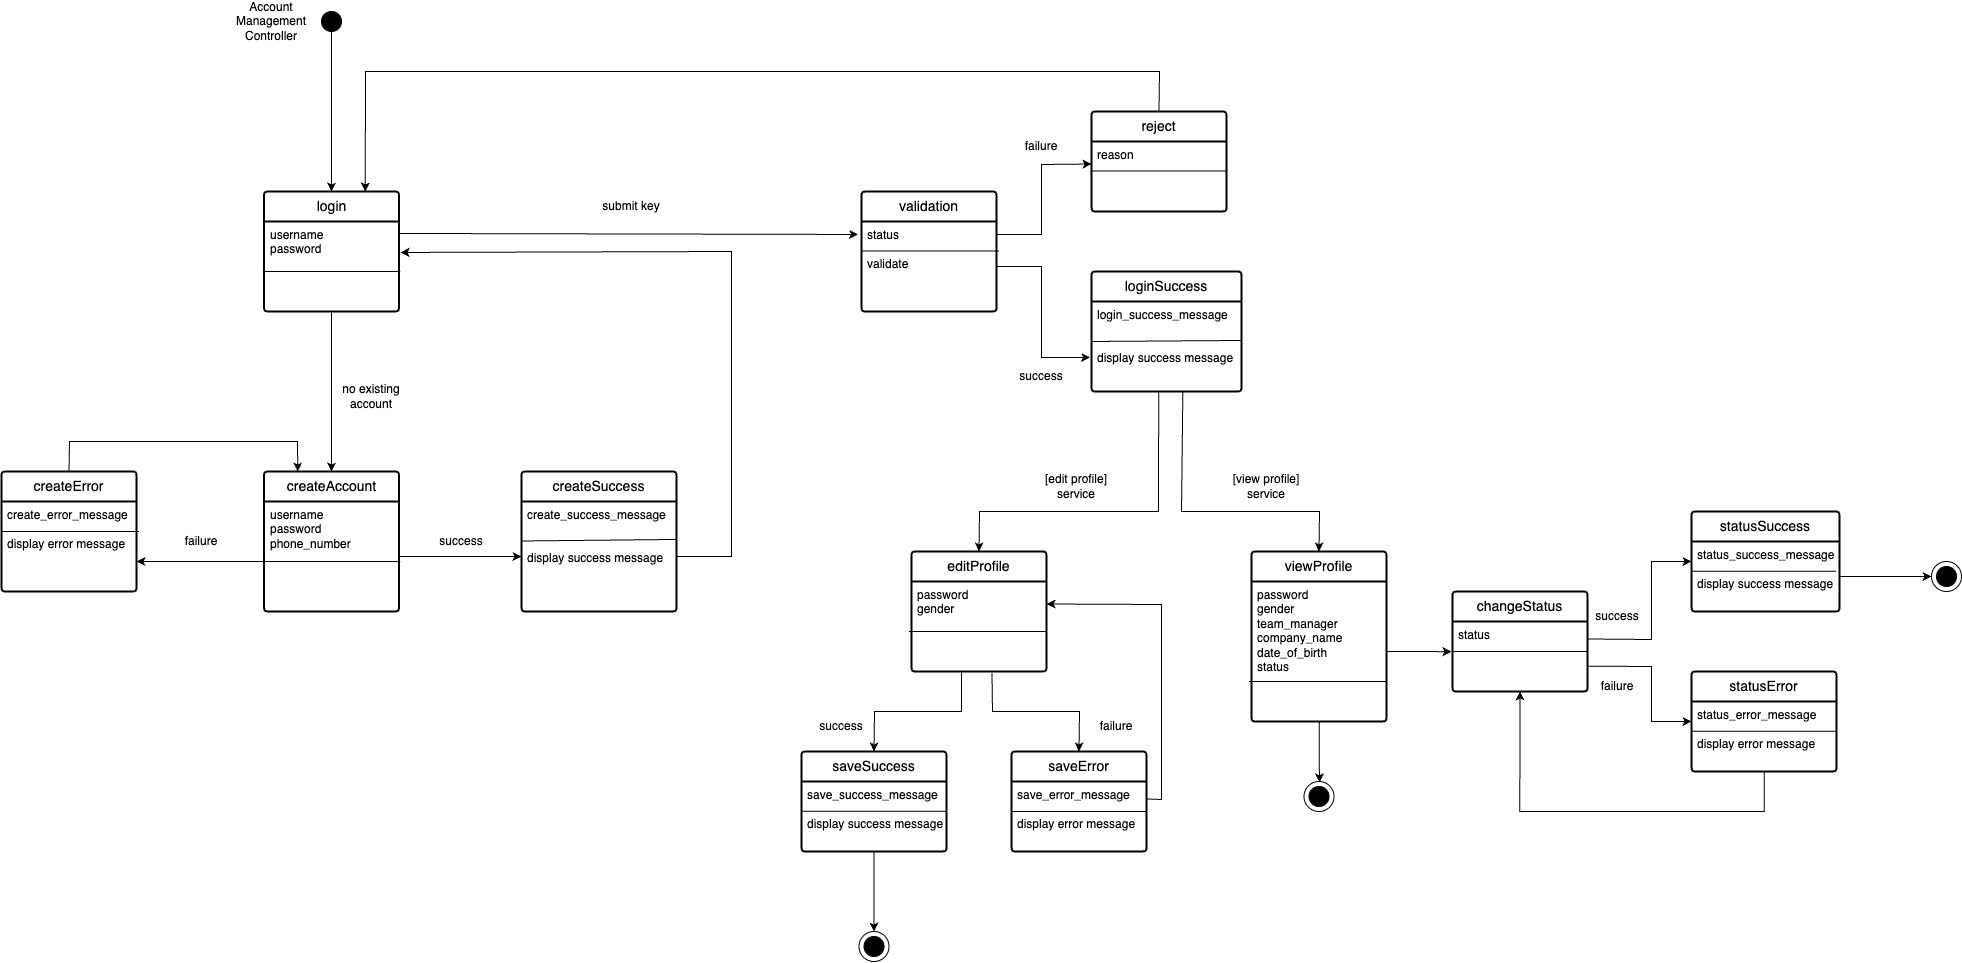
\includegraphics[scale=0.25]{account-controller.jpg}
    \caption{Overall Account Management Controller State Diagram}
    \label{fig:account-controller}
\end{figure}

\begin{figure}[H]
    \centering
    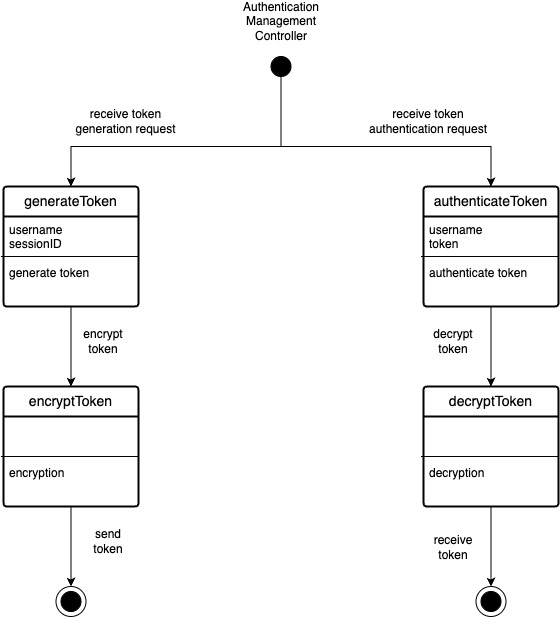
\includegraphics[scale=0.75]{authenticaton-controller.jpg}
    \caption{Overall Authentication Management Controller State Diagram}
    \label{fig:authentication-controller}
\end{figure}
% End Section


\section{Sequence Diagrams}
\label{sec:sequence_diagrams}
% Begin Section

%\textbf{BE1: Authorizing Employees}

\begin{figure}[H]
    \centering
    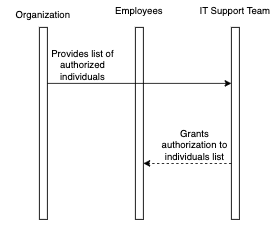
\includegraphics[width=7cm]{BE1.png}
    \caption{BE1 - Authorizing Employees}
    \label{fig:galaxy}
\end{figure}

%\textbf{BE2: Login}
\vspace{1 cm}
\begin{figure}[H]
    \centering
    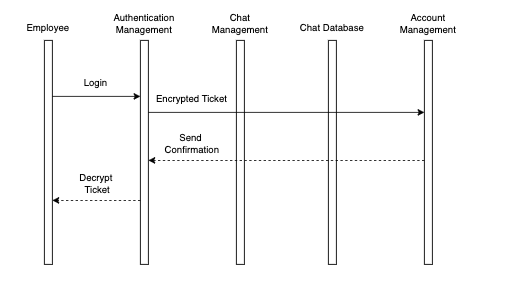
\includegraphics[width=11cm]{BE2.png}
    \caption{BE2 - Login}
    \label{fig:galaxy}
\end{figure}


%\textbf{BE3: Creating Individual Chat Threads}

\begin{figure}[H]
    \centering
    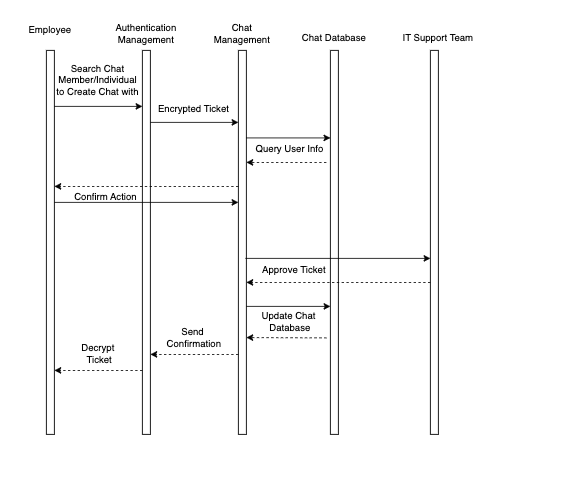
\includegraphics[width=10cm]{BE3.png}
    \caption{BE3 - Creating Individual Chat Threads}
    \label{fig:galaxy}
\end{figure}

%\textbf{BE4: Creating Group Chat Threads}

\begin{figure}[H]
    \centering
    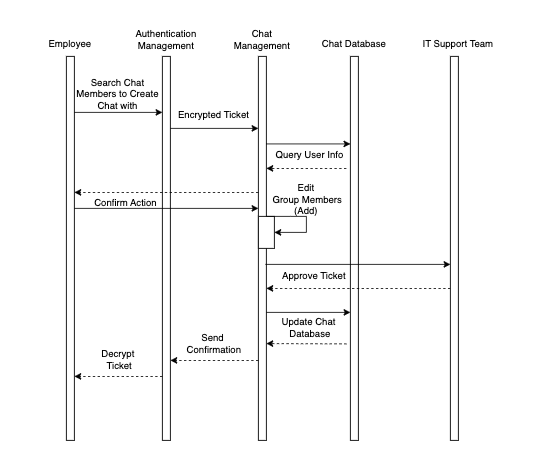
\includegraphics[width=10cm]{BE4.png}
    \caption{BE4 - Creating Group Chat Threads}
    \label{fig:galaxy}
\end{figure}

%\textbf{BE5: Sending Text-Only Chats}

\begin{figure}[H]
    \centering
    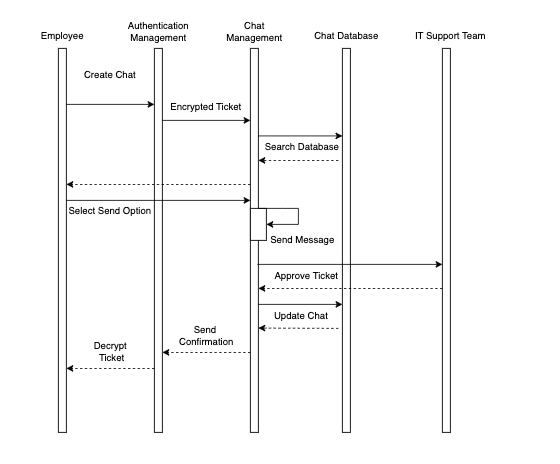
\includegraphics[width=10cm]{BE5.png}
    \caption{BE5 - Sending Text-Only Chats}
    \label{fig:galaxy}
\end{figure}
\hspace{1cm}

%\textbf{BE6: Sending File Attachments}

\begin{figure}[H]
    \centering
    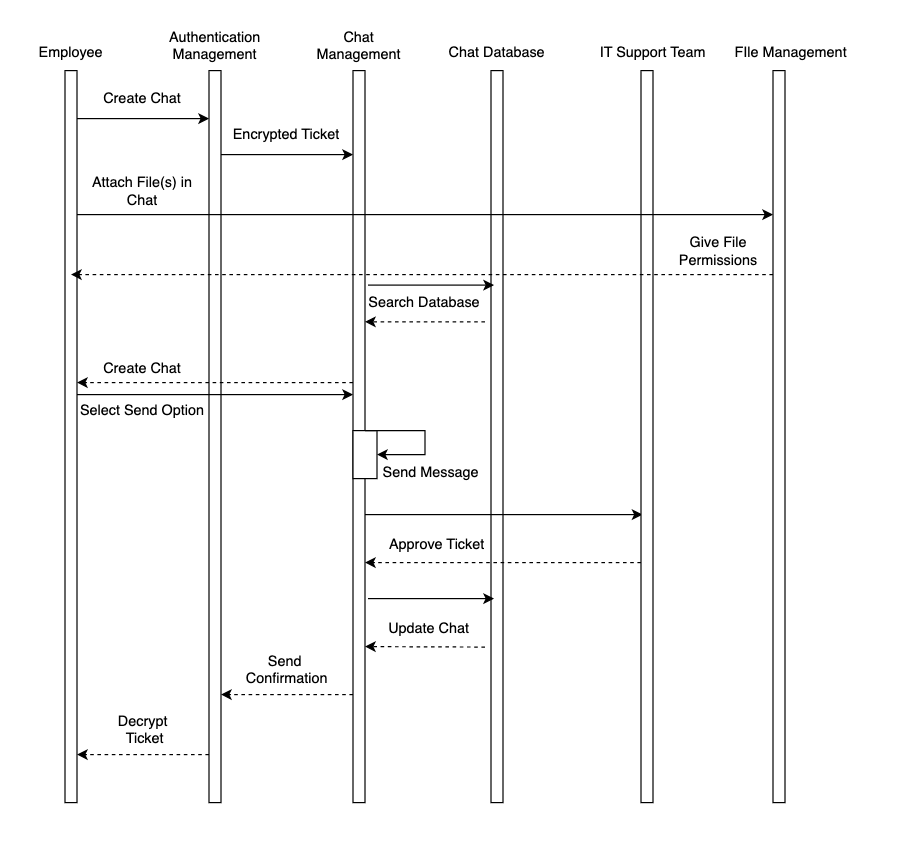
\includegraphics[width=9cm]{BE6.png}
    \caption{BE6 - Sending File Attachments}
    \label{fig:galaxy}
\end{figure}

\begin{figure}[H]
	\centering
	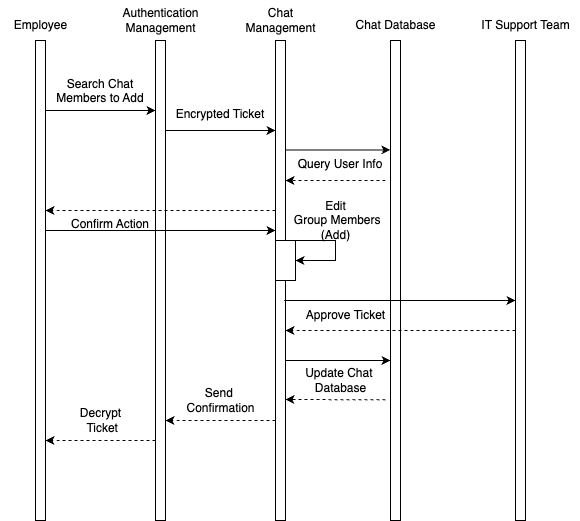
\includegraphics[width=0.8\textwidth]{BE7.png}
	\caption{Add Individuals to Chat Sequence Diagram}
\end{figure}

\begin{figure}[H]
	\centering
	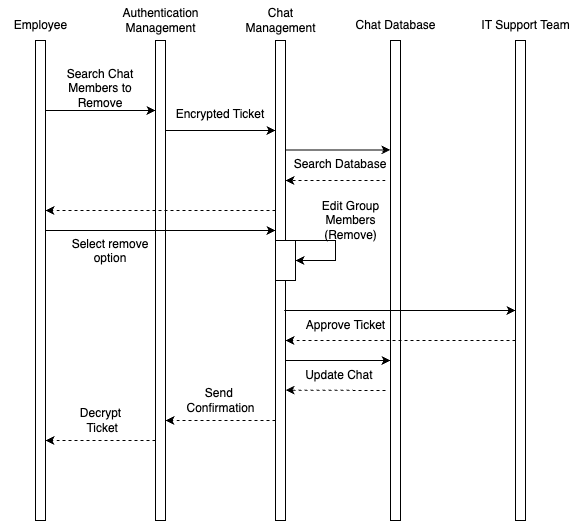
\includegraphics[width=0.8\textwidth]{BE8.png}
	\caption{Remove Individuals to Chat Sequence Diagram}
\end{figure}

\begin{figure}[H]
	\centering
	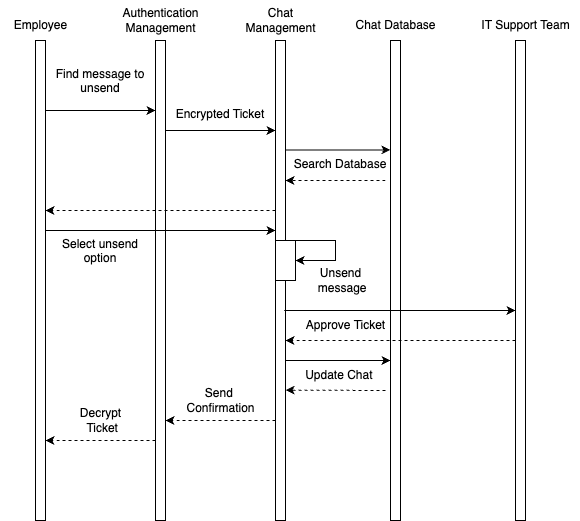
\includegraphics[width=0.8\textwidth]{BE9.png}
	\caption{Delete Message Sequence Diagram}
\end{figure}

\begin{figure}[H]
	\centering
	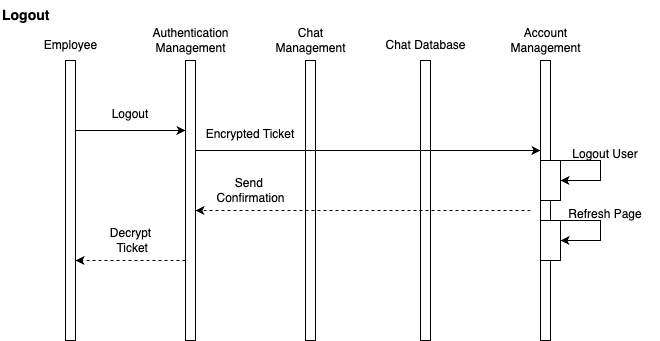
\includegraphics[width=0.8\textwidth]{BE10.png}
	\caption{Logout Sequence Diagram}
\end{figure}

\begin{figure}[H]
	\centering
	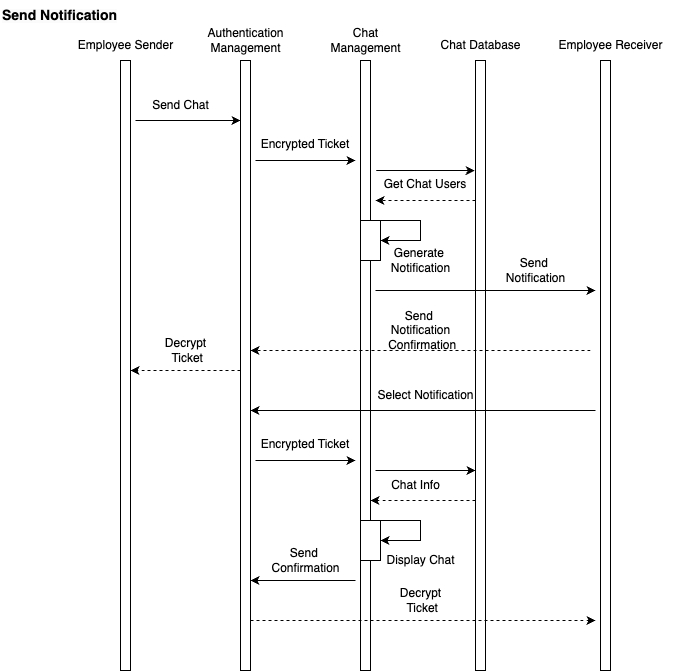
\includegraphics[width=0.8\textwidth]{BE11.png}
	\caption{Send Notification Sequence Diagram}
\end{figure}


% End Section


\section{Detailed Class Diagram}
\label{sec:detailed_class_diagram}
% Begin Section
\renewcommand{\thefigure}{4.\arabic{figure}}
\setcounter{figure}{0}
\begin{figure}
    \centering
    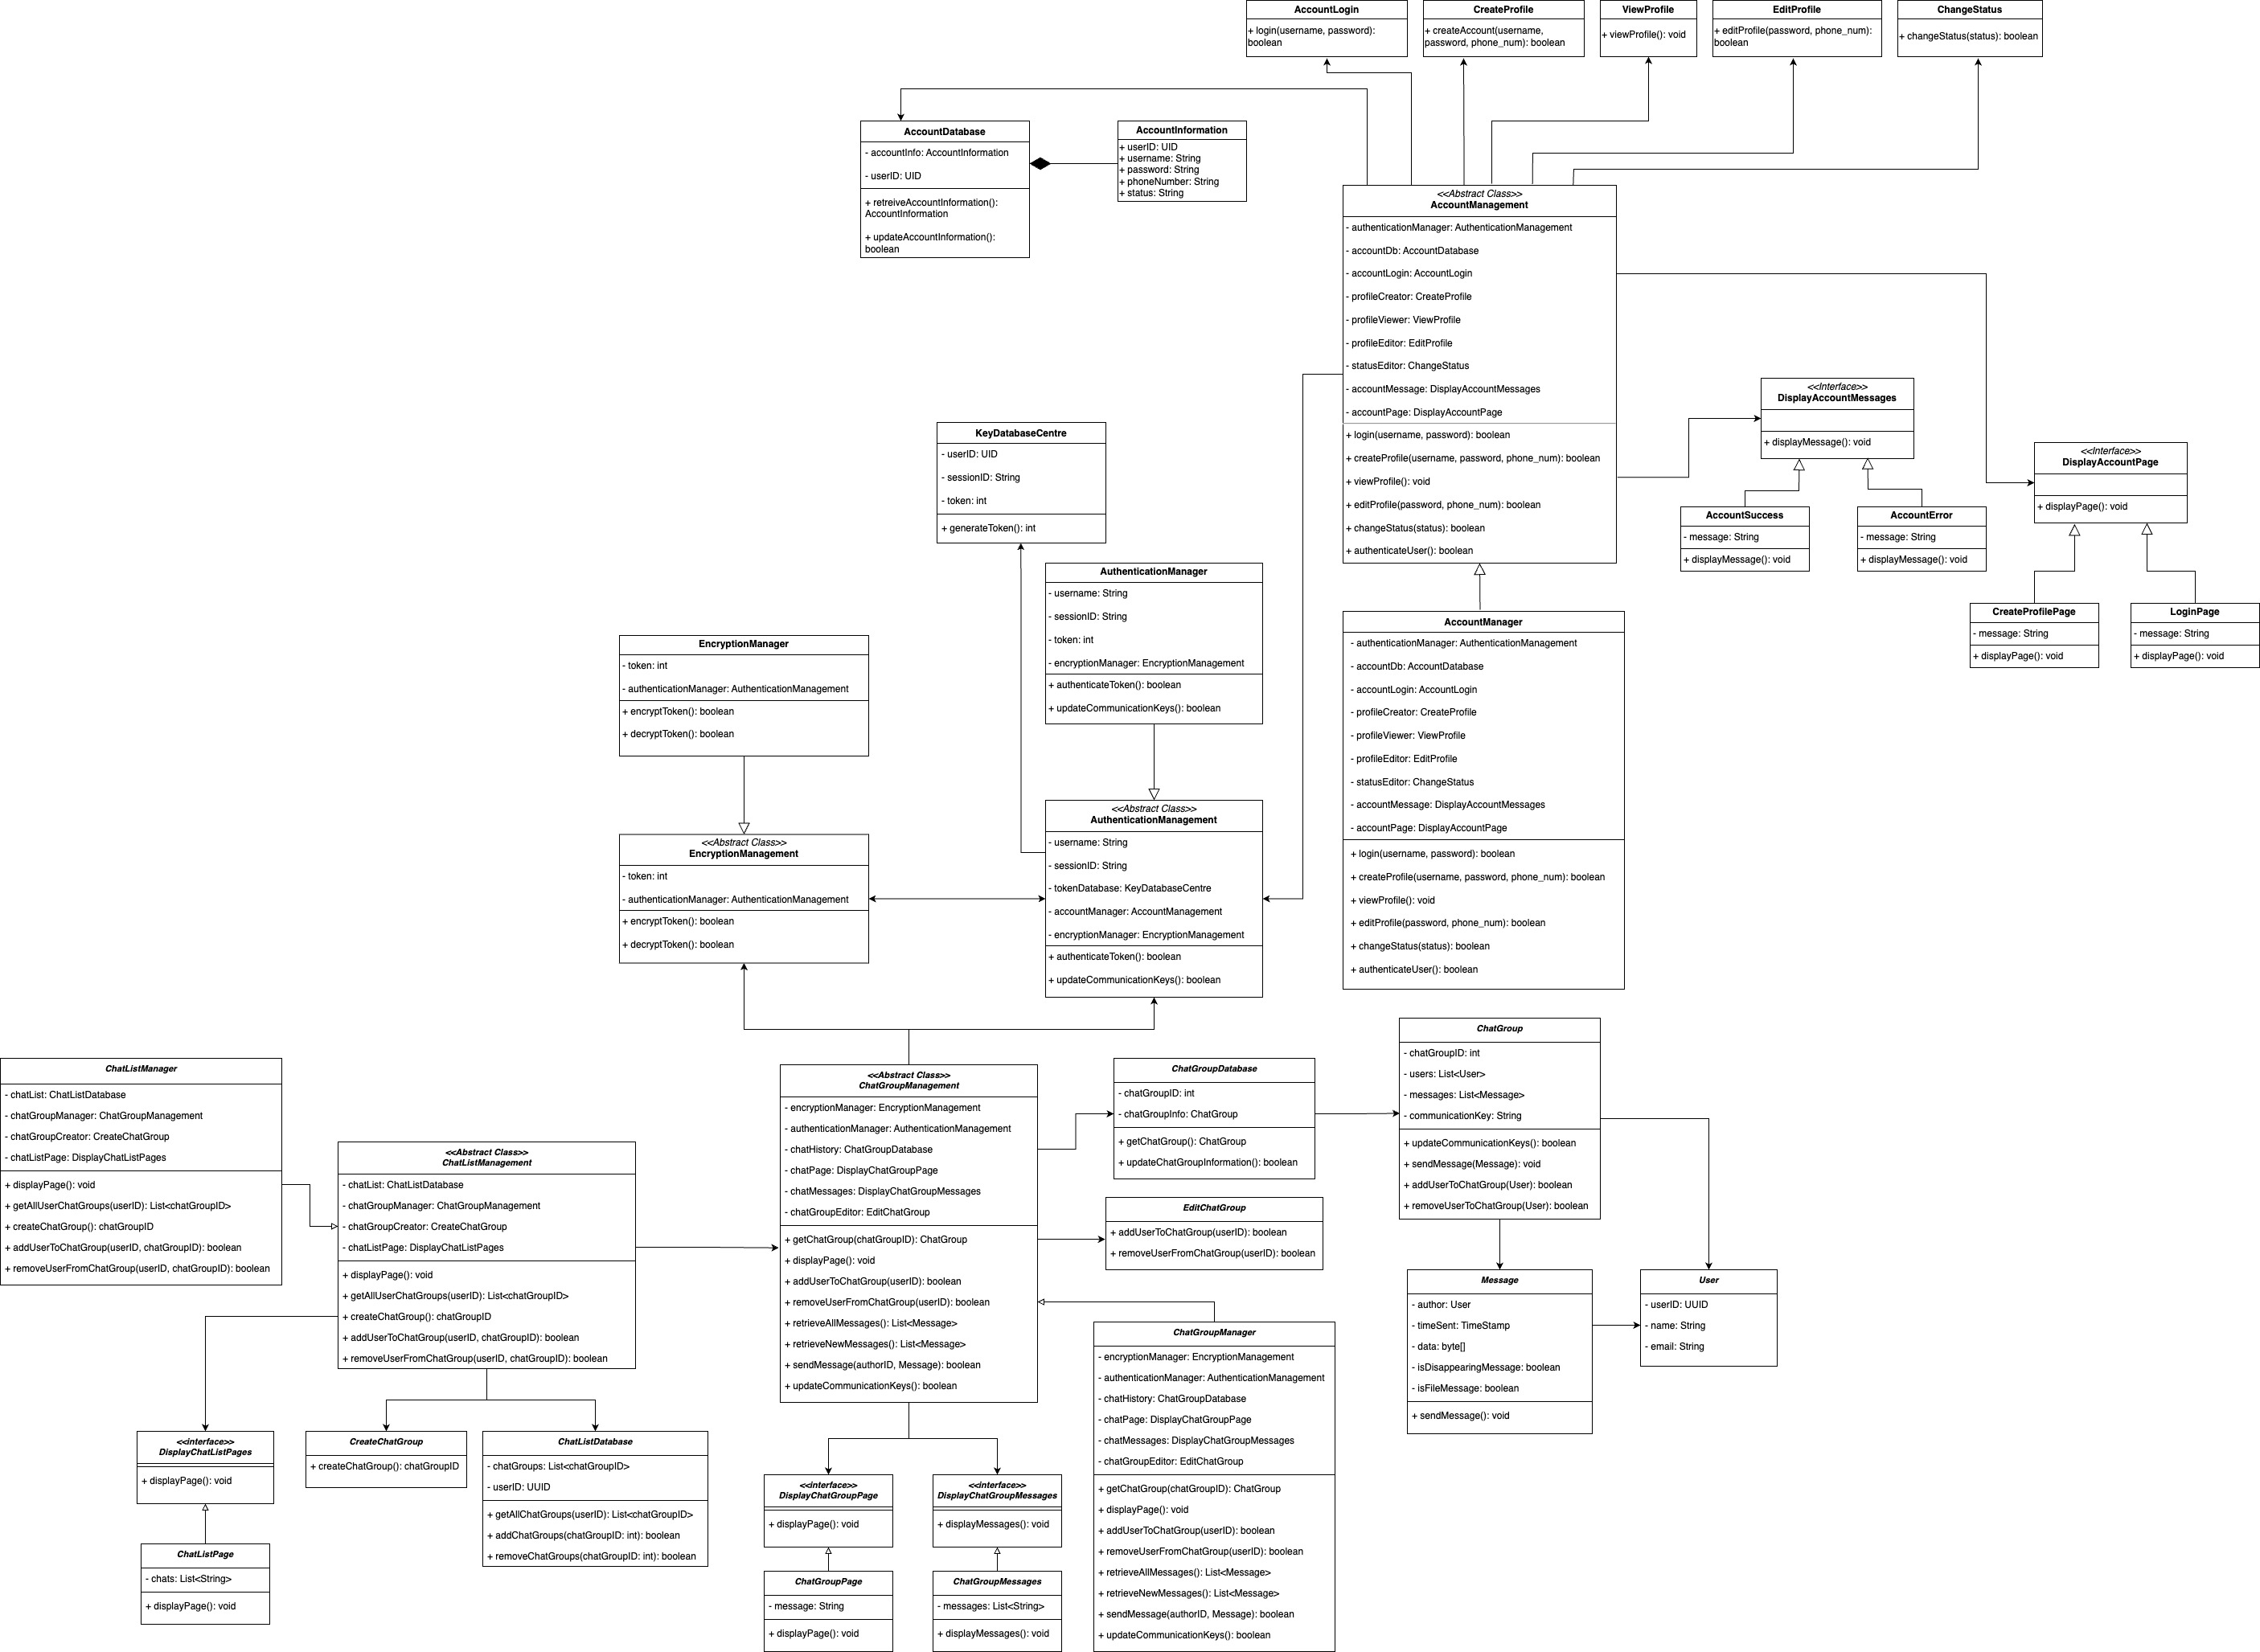
\includegraphics[scale=0.18]{class-diagram.jpg}
    \caption{Overall Class Diagram}
    \label{fig:class-diagram}
\end{figure}
% End Section



\appendix
\section{Division of Labour}
\label{sec:division_of_labour}
% Begin Section
Include a Division of Labour sheet which indicates the contributions of each team member. This sheet must be signed by all team members.
% End Section
\subsection{Awurama Nyarko}
\label{subsec:awurama_nyarko}
\begin{itemize}
	\item 1.1 Purpose
	\item 1.2 System Description
	\item 1.3 Overview
 	\item Figure 2.1 State Diagram for Chat Management Controller Class
  	\item Figure 2.2 State Diagram for File Management Controller Class
\end{itemize}
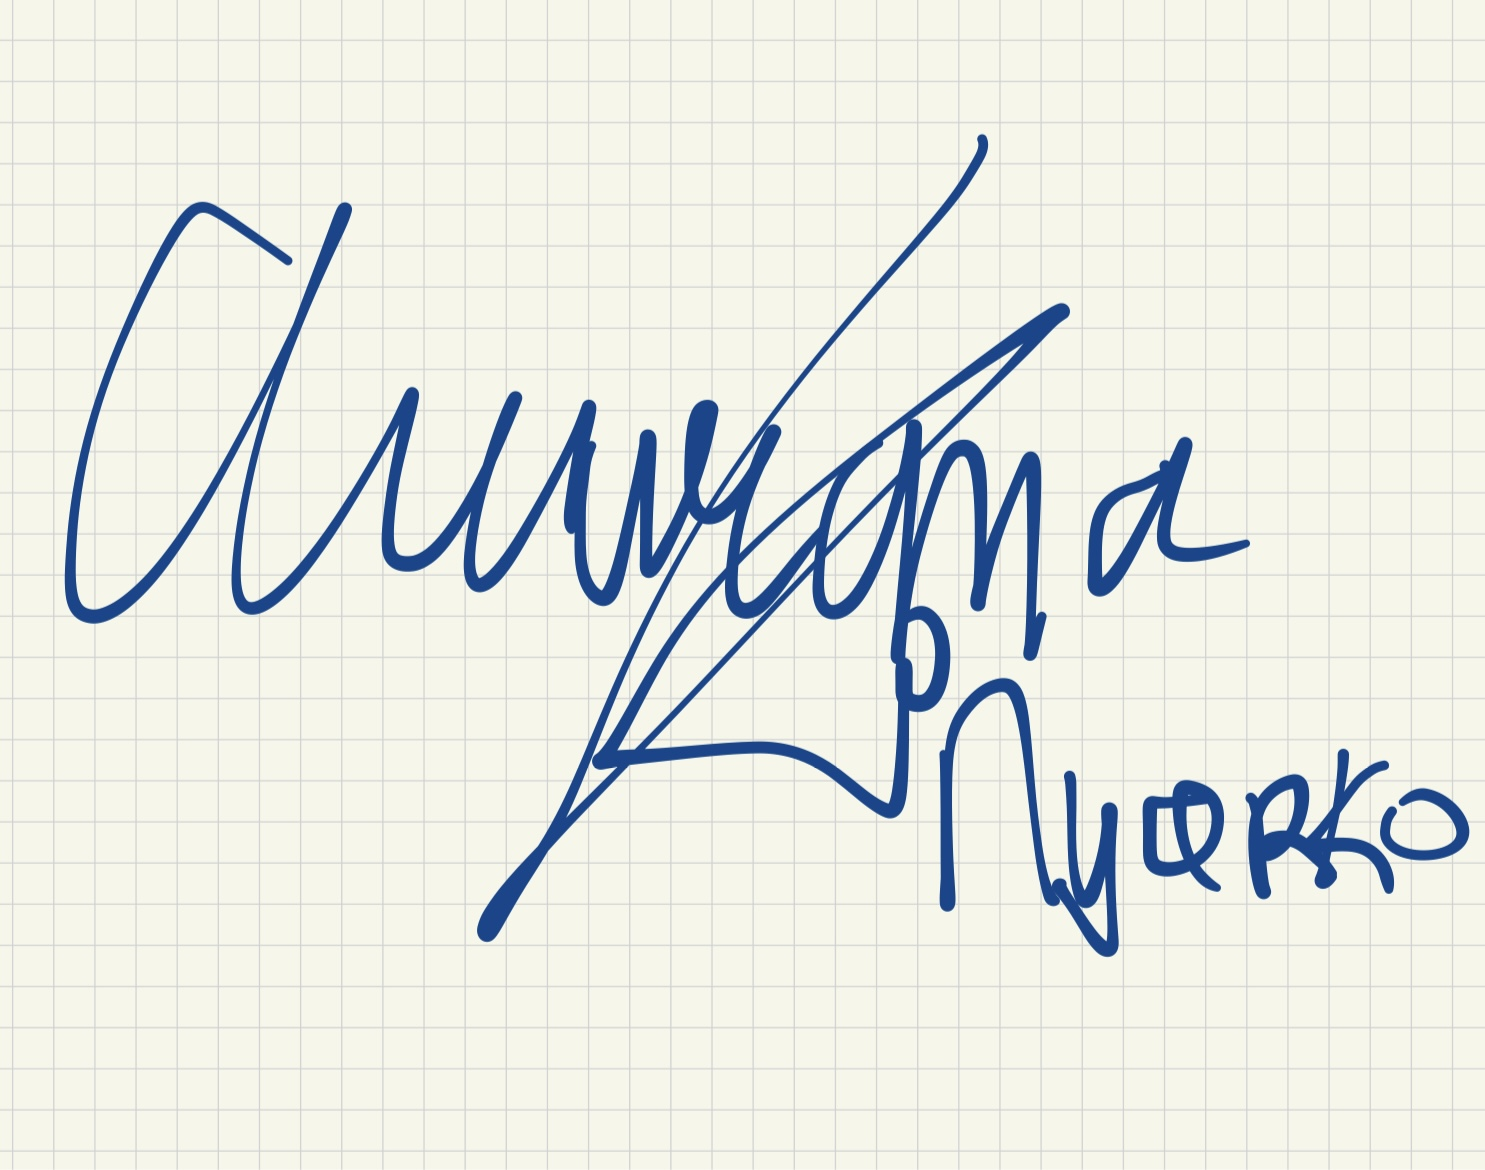
\includegraphics[width=0.5\textwidth]{awurama.jpg}

\subsection{Chelsea Maramot}
\label{subsec:chelsea_maramot}
\begin{itemize}
	\item Sequence Diagrams
 		\begin{itemize}
   			\item Figure 3.7 Adding Individals to Group (BE7)
      			\item Figure 3.8 Removing Individuals from Group (BE8)
	 		\item Figure 3.9 Unsending a Chat/Communication (BE9)
    			\item Figure 3.10 Signing out of the Chat Application (BE10)
       			\item Figure 3.11 Notifications being sent to Users (BE11)
      		\end{itemize}
\end{itemize}
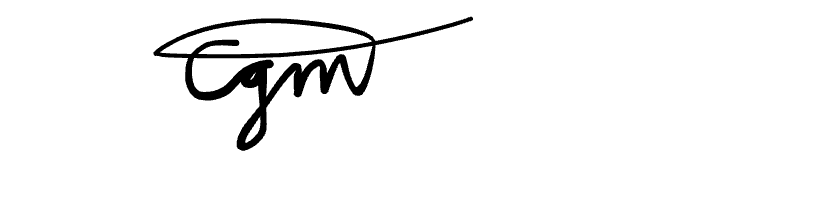
\includegraphics[width=0.5\textwidth]{chelsea.png}

\subsection{Harrison Chiu}
\label{subsec:harrison_chiu}
\begin{itemize}
	\item Figure 4.1 Overall Class Diagram
 		\begin{itemize}
   			\item Chat Management and related classes
      			\item File Management and related classes
	 	\end{itemize}
\end{itemize}

\includegraphics[width=0.5\textwidth]{harrison.png}

\subsection{Khushi Bhojane}
\label{subsec:khushi_bhojane}
\begin{itemize}
	\item Sequence Diagrams
 		\begin{itemize}
   			\item Figure 3.1 Authorizing (BE1)
      			\item Figure 3.2 Login (BE2)
	 		\item Figure 3.3 Create Individual Chat Thread (BE3)
    			\item Figure 3.4 Create Group Chat (BE4)
       			\item Figure 3.5 Send Text Only Message (BE5)
	  		\item Figure 3.6 Send Files (BE6)
      		\end{itemize}
\end{itemize}

\includegraphics[width=0.5\textwidth]{khushi_signature.png}

\subsection{Sumanya Gulati}
\label{subsec:sumanya_gulati}
\begin{itemize}
	\item Figure 2.3 State Diagram for Account Management Controller Class
 	\item Figure 2.4 State Diagram for Authentication Management Controller Class
	\item Overall Class Diagram
 		\begin{itemize}
   			\item Account Management and related classes
      			\item Authentication Management and related classes
      		\end{itemize}
	\item Division of Labour
\end{itemize}

\includegraphics[width=0.5\textwidth]{signature.jpeg}

\newpage
\section*{IMPORTANT NOTES}
\begin{itemize}
	\item You do \underline{NOT} need to provide a text explanation of each diagram; the diagram should speak for itself
	\item Please document any non-standard notations that you may have used
	\begin{itemize}
		\item \emph{Rule of Thumb}: if you feel there is any doubt surrounding the meaning of your notations, document them
	\end{itemize}
	\item Some diagrams may be difficult to fit into one page
	\begin{itemize}
		\item It is OK if the text is small but please ensure that it is readable when printed
		\item If you need to break a diagram onto multiple pages, please adopt a system of doing so and throughly explain how it can be reconnected from one page to the next; if you are unsure about this, please ask me
	\end{itemize}
	\item Please submit the latest version of Deliverable 1 and Deliverable 2 with Deliverable 3
	\begin{itemize}
		\item They do not have to be a freshly printed versions; the latest marked versions are OK
	\end{itemize}
	\item If you do \underline{NOT} have a Division of Labour sheet, your deliverable will \underline{NOT} be marked
\end{itemize}


\end{document}
